\documentclass{article}
\usepackage[utf8]{inputenc}
\usepackage{natbib}
\usepackage{graphicx, caption, amsmath, amssymb, subcaption}
\newcommand*{\myfont}{\fontfamily{lmtt}\selectfont}
\title{PhyloDivNet}
\author{Trinh & Willis}
\date{June 2019}


\begin{document}
\maketitle
\section{Introduction}
- Talk about beta-diversity and why we analyze microbiome data in this way.

- Talk about UniFrac and its differenct flavors of weighted/unweighted.
- UniFrac has not traditionally been discussed as an estimand. First time UnIFrac and estimand are even referred to in the a sentence.
- Bacteria are networked and as such DivNet and by extension PhyloDivNet provides a way to incorporate the network structure in our phylogenetic beta-diversity estimation
- The way this paper distinguishes itself is through a robust look at the pairing of the log-ratio model for estimating relative abundances (which we know DivNet is a good estimator of non-phylogenetic diversity metrics) with the phylogenetic tree in estimating UniFrac. Basically we really need to find situations in which this proposed method might be limited so that would require me to really look at different tree structures more carefully.
-
Outline:
\begin{itemize}
  \item  If people want to make inferential estimates of individual-level pairwise UniFracs then they need to incorporate biological replicates.
  \item  Bacteria are networked and as such DivNet and by extension PhyloDivNet provides a way to incorporate the network structure in our phylogenetic beta-diversity estimation
  \item  Talk about UniFrac and how it has a weighted and unweighted version. Here PhyloDivNet is appropriate for weighted UniFrac because we are testing group differences and as such there's a pooling of information that occurs for inferring some mean group relative abundances for each taxon. Because unweighted UniFrac is a phylogenetic quantitative measure that uses presence/absence information, this approach is not well suited for that metric.
  \item  Segue into the use of PhyloDivNet and its advantages, particularly when evaluating its performance in hypothesis testing
\end{itemize}


\section{Estimating Weighted UniFrac}

Weighted UniFrac is a quantitative phylogenetic diversity index and as such utilizes abundance information and a phylogenetic tree in its calculation. We start with samples from $i = 1,..., n$ ecosystems that have a known vector of covariates $X_i \in R^p$. $Q$ represents the number of species present in one or more ecosystems and we use $q = 1,...,Q$ to index the $Q$ taxa across all ecosystems. $Z_{iq} [0,1]$ refers to the latent relative abundance of taxon $q$ in ecosystem $i$ with the relative abundances of all taxon $q$ in ecosystem $i$ summing to 1. For each ecosystem $i$ there are $M_i$ total sequence counts observed that have been classified into $q$ taxa. $W_{iq}$ will represent the number of observed counts of taxon $q$ in ecosystem $i$.

For the phylogenetic tree, let $m = 1,..., M$ index the branches of the phylogenetic tree where $M$ represents the total number of branches of the phylogenetic tree. $b_m$ denotes the branch length of the $nth$ branch. $d$ is the distance from each taxon $q$ to the root. And let $S_m$ represent the set of taxa that are descendents from branch $m$.

The weighted UniFrac (Lozupone et. al 2007) diversity metric is defined as
\begin{equation}
    \hat{\beta}_{ij,WU,plug-in}=\sum_{i=1}^n b_n |\sum_{q \in S_{in}} \frac{W_{iq}}{M_i}-\sum_{q \in S_{jn}} \frac{W_{jq}}{M_j}|
\end{equation}
Based on Eq. 1, the target estimand for weighted UniFrac is
\begin{equation}
    \beta_{ij,WU}=\sum_{i=1}^n b_n |\sum_{q \in S_{in}} Z_{iq} -\sum_{q \in S_{jn}} Z_{jq}|
\end{equation}
To our knowledge, there has been no discussion of the target estimand for weighted UniFrac in the literature to date. There also exists a normalized weighted UniFrac metric where $\beta_{ij,WU} \in [0,1]$.  The normalized UniFrac plug-in estimate divides the weighted UniFrac by the average distance of each taxon $q$ from the root.
\begin{equation}\label{eq:plugin}
    \hat{\beta}_{ij,NWU,plug-in}=\frac{\sum_{i=1}^n b_n |\sum_{q \in S_{in}} \frac{W_{iq}}{M_i}-\sum_{q \in S_{jn}} \frac{W_{jq}}{M_j}|}{\sum_{q=1}^Q d_q (\frac{W_{iq}}{M_i}+\frac{W_{jq}}{M_j})}
\end{equation}
The target estimand for normalized weighted UniFrac is therefore
\begin{equation}
    \beta_{ij,NWU}=\frac{\sum_{i=1}^n b_n |\sum_{q \in S_{in}} Z_{iq}-\sum_{q \in S_{jn}} Z_{jq}|}{\sum_{q=1}^Q d_q (Z_{iq}+Z_{jq})}
\end{equation}

Compositional data can be modeled using a multinomial distribution where the covariances between components are negative constrained. If the sum of all components is equal to some known fixed $n$, an increase in one component will result in a decrease in another component and therefore be negatively correlated. To address this negative constrained covariance issue we follow the {\myfont DivNet}(Willis and Martin[under review]) approach to estimating the latent composition matrix $Z \in R^{nxQ}$ and beta-diversity. {\myfont DivNet} uses Aitchison’s log-ratio methodology to estimate the latent composition matrix by first modeling $W_{iq}$ from a multinomial distribution,
\begin{equation}
p(W|Z)\propto\prod_{i=1}^n \prod_{q=1}^Q Z_{iq}^{W_{iq}}
\end{equation}
and then performing the log-ratio transformation by fixing some baseline taxon D as a comparison group:
\begin{equation}
    Y_{iq}=\phi{Z_{iq}}=\{log(\frac{Z_{iq}}{Z_{iD}})\}_{q=1,...,D-1,D+1,...Q}
\end{equation}
Note that the log-ratio transformation is invertible $Z_{iq}=\phi^{-1}{Y_{iq}}$. The log-ratios $Y_{i}$ are then modeled using a multivariate normal distribution. We link the mean of $Y_i$ to covariates using $\mu_{i}=X_{i}^T\beta$. Our expected value of $Y_i$ can therefore be expressed as
\begin{equation}
    \hat{Y_i} = X_{i}^T \hat{\beta}
\end{equation}
where $\hat{\beta}$ is the maximum likelihood estimate of $\beta$. The expected value of our random variable $Y_i$ can then be used to derive the fitted values of the latent composition since $\hat{Z}_i=\phi^{-1}(Y_i)$.

Using {\myfont DivNet}'s estimation approach of $\beta$-diversity we propose the following estimate of weighted UniFrac and normalized weighted UniFrac
\begin{equation}
\hat{\beta}_{ij,WU,proposed}=\sum_{i=1}^n b_n |\sum_{q \in S_{in}} \hat{Z}_{iq} -\sum_{q \in S_{jn}} \hat{Z}_{jq}|
\end{equation}
\begin{equation}
    \hat{\beta}_{ij,NWU,propose}=\frac{\sum_{i=1}^n b_n |\sum_{q \in S_{in}} \hat{Z}_{iq}-\sum_{q \in S_{jn}} \hat{Z}_{jq}|}{\sum_{q=1}^Q d_q (\hat{Z}_{iq}+\hat{Z}_{jq})}
\end{equation}

For the phylogenetic tree, we assume that the phylogenetic tree that is constructed is correctly specified. Here we define an estimand for weighted UniFrac and a proposed method which we call {\myfont PhyloDivNet} for estimating the weighted UniFrac estimand.

\section{Variance Estimation}
Accurate estimation of the variance of UniFrac estimates has important implications towards valid hypothesis testing. Variance estimation of our UniFrac estimates is carried out using parametric and nonparametric bootstrap approaches and evaluated under simulation.
Parametric bootstrapping to estimate the $Var(\widehat{UniFrac_{ij}})$ is conducted as follows:
Let $\hat{\beta}$ and $\hat{\Sigma}$ be the estimates of $\beta$ and $\Sigma$ of our log-ratio model and $B$ represent the number of bootstrap iterations. We simulate $B$ number of datasets from the log-ratio model using our $\hat{\beta}$ and $\hat{\Sigma}$ estimates.  For each simulated dataset $b=1,...,B$ we use {\myfont DivNet} to estimate the $\hat{\beta}^{b}$ and $\hat{\Sigma}^{b}$. From there,  we estimate the weighted UniFrac ($\widehat{UniFrac}_{ij}^{b}$) for $b=1,...,B$. The $\widehat{Var}(\widehat{UniFrac_{ij}^{b}})$ is therefore the parametric bootstrap estimate of the $Var(\widehat{UniFrac_{ij}})$.

Nonparametric bootstrapping to estimate the $Var(\widehat{UniFrac_{ij}})$ begins with some dataset $(W,X)$. We define $n_{sub}$ as the number of samples we want to subsample from the dataset (W,X) and let $i = 1,...,I$ index the samples. We then use a uniform random selection of $n_{sub}$ elements from ${1,...,n_{sub}}$ that will correspond to the sample indices subsampled from some dataset $(W,X)$. The subsampled set of samples will be referred to as $P$. With each set $P$ we estimate $\hat{\beta}^{P}$ and $\hat{\Sigma}^{P}$ to obtain $\widehat{UniFrac_{ij}^{P}}$. We repeat this subsampling from (W,X) and estimation of $\widehat{UniFrac_{ij}^{P}}$ for $B$ iterations until we obtain a set of UniFrac estimates $\widehat{UniFrac_{ij}^{P_{b}}}$ for $b = 1,...,B$ bootstrap iterations. From there we obtain the nonparametric bootstrap estimate of $Var(\widehat{UniFrac_{ij}})$ by calculating $\widehat{Var}(\widehat{UniFrac_{ij}^{P_{b}}})$.

\subsection{Variance Estimation Simulation Study}
As mentioned by Willis and Martin [Under Review], $q>>n$ in microbiome studies and as such the generalized inverse approach may inappropriate for estimating the inverse covariance. Willis and Martin therefore compared several approaches to estimate the inverse covariance such as using a regularize estimate from the graphical lasso, a maximum likelihood estimate restricted to the diagonal covariance matrices, and the generalized inverse of the sample covariances. They found that there was no substantial advantage in estimating the inverse covariance between any of the three approaches and as such we choose the generalized inverse of the sample covariances approach as our method for estimating the inverse covariance in our variance estimation simulations.

We compare both nonparametric and parametric bootstrapping approaches to estimating $Var(\widehat{UniFrac_{ij}})$ under simulation. We simulate our data from a log-ratio model by specifying $\beta, \Sigma$, $X$, and $M$. $\beta$ is generated from a random normal distribution with $\mu = 0$ and $SD = 1$. $\Sigma$ is constructed by first creating a matrix $A \in \mathbb{R}^{(Q-1)(Q-1)}$ whose elements are drawn from a uniform distribution that range from (-1,1). From there a diagonal matrix $D$ is created where the diagonal elements are an arithmetic sequence of length $Q$ starting from $\sigma_{max}$ and ending at $\sigma_{min}$. $\Sigma$ is then calculated as $\Sigma = A^{T}DA$.  $X =(1_n^{T}, (0_{n/2},1_{n/2})^{T},(0,1)_{n/2}^{T})$ and $M$ is the sequencing depth for each ecosystem $i$ set to 10,000. We fix $n = 30$, $\sigma_{min}=0.01$, $\sigma_{max}= 5$, and evaluate varying $Q = 20, 50, 100$ for 50 simulations under a log-ratio model. To simulate from the log-ratio model with specified parameters $\beta, \Sigma, X, M$, we simulate a matrix $Y_i$ from a  $N(X_{i}^{T}\beta,\Sigma)$ then calculate $Z_i = \phi^-1(Y_i)$ for the $i$th row to obtain the $Z$ matrix. With the $Z$ matrix we can simulate our count data $W_i$ from a $Multinomial(M_i,Z_i)$. We select $B$ = 3 iterations for the parametric bootstrap and $B$ = 3 subsamples of $n_{sub}$ = 26 samples for the nonparametric bootstrap.

\begin{figure}[!htb]
  \captionsetup{singlelinecheck = false, format= hang, justification = raggedright, font = sf, labelsep = space}
   \caption{Variance Estimation Results}
  \centering
    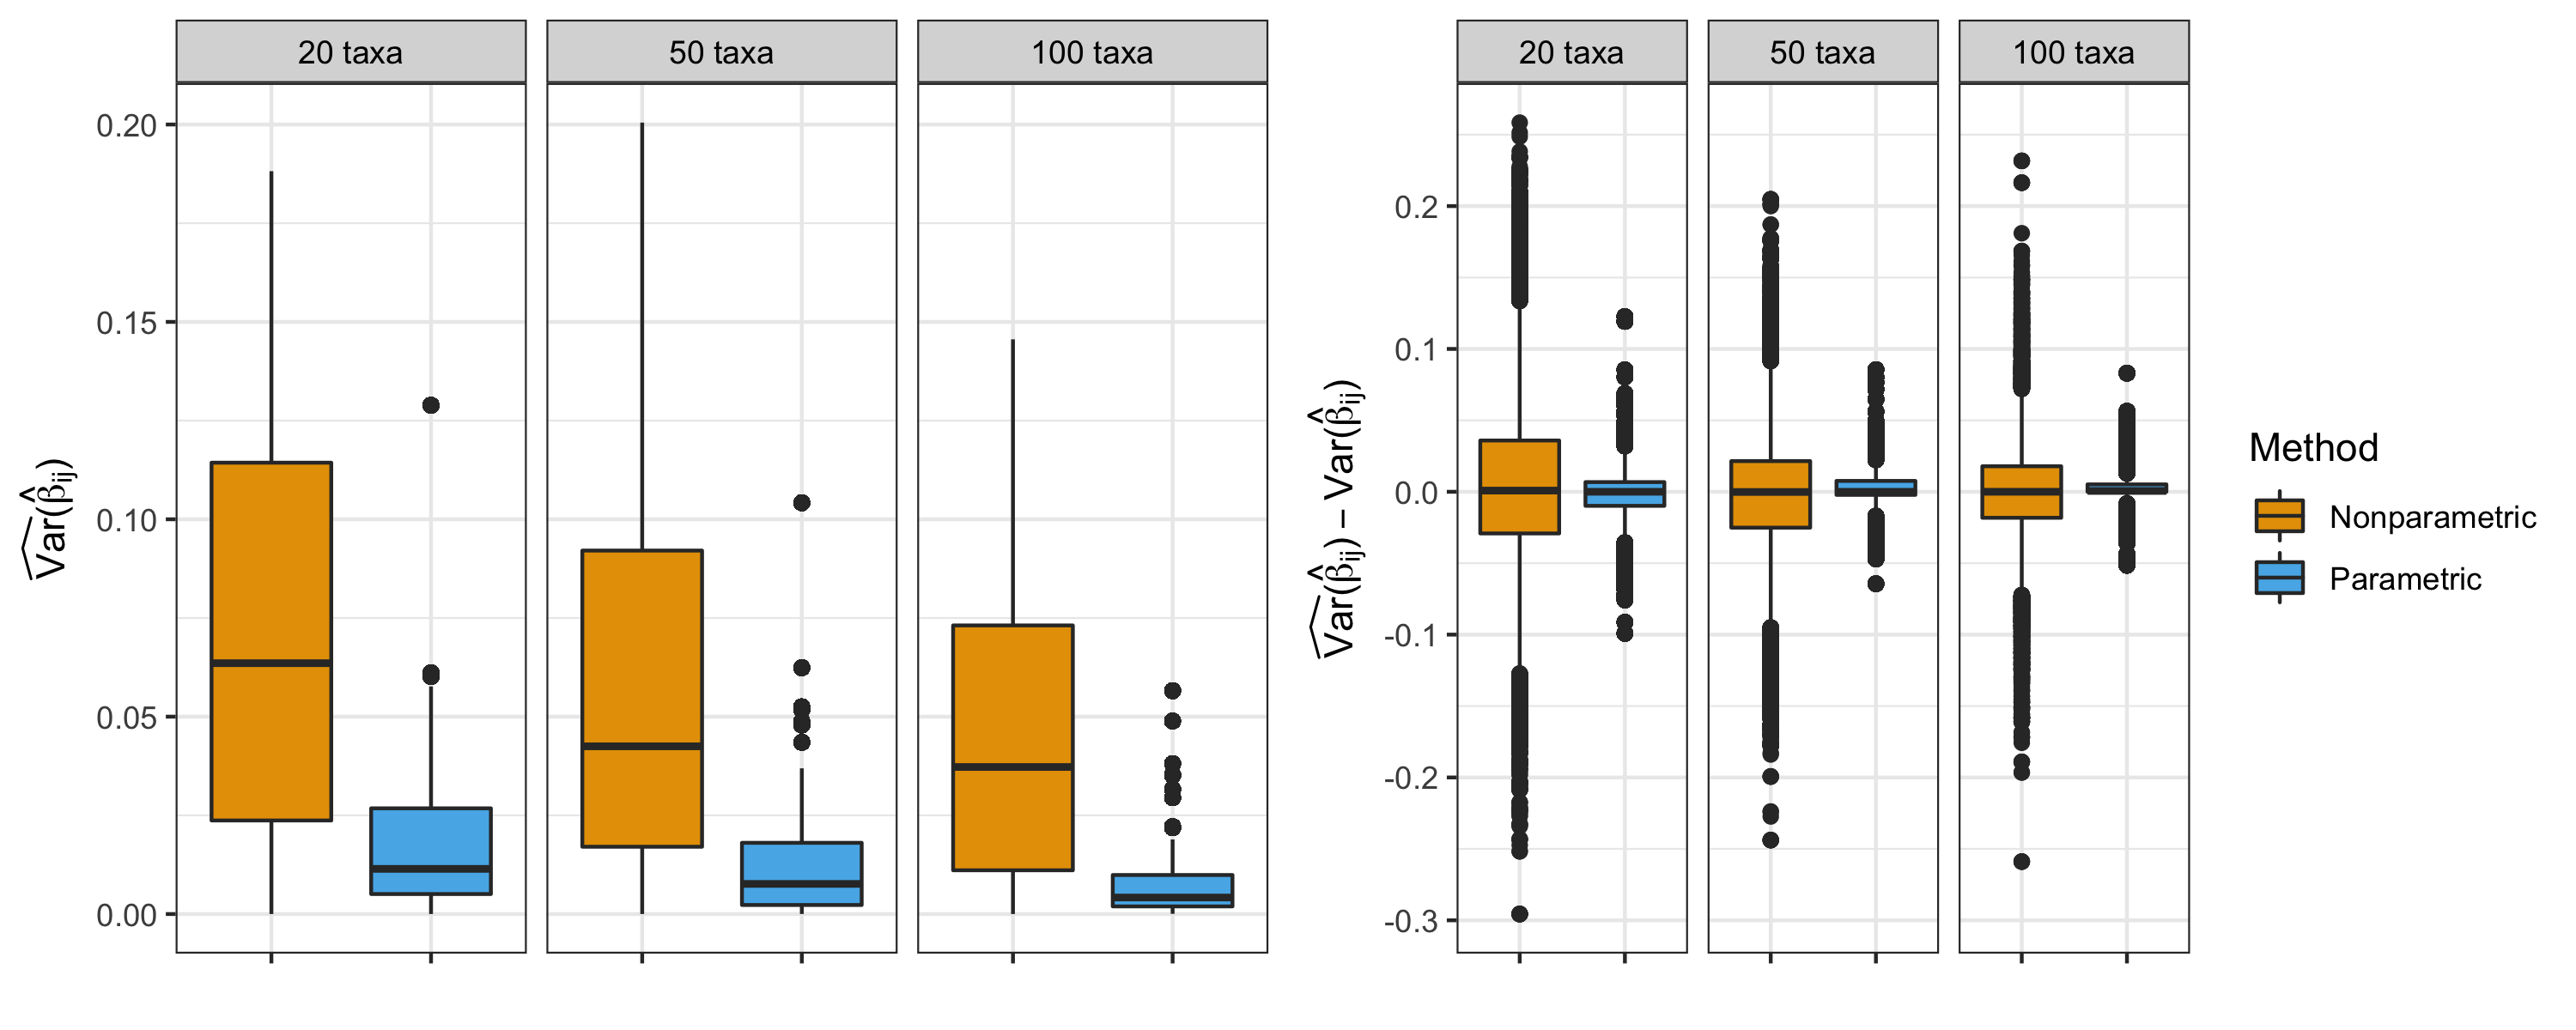
\includegraphics[width=\textwidth]{variance_plots2.png}
\end{figure}

Results from our simulations are displayed in Figure 1. We observe that the parametric bootstrap variances have a lower median estimated variance for all $Q$ with increasing number of taxa resulting in lowering median estimated variances for both the nonparametric and parametric bootstrap approaches (left panel). We present the difference between the estimated variance and the true variance for both approaches in the right panel. The true variance was estimated by simulating data according to ($\beta$, $\Sigma$, and $M$), calculating the weighted UniFrac for each dataset, then calculating the variance of the weighted UniFrac estimates. We see that the median difference between our estimated variance and the true variance is closer to zero for the parametric bootstrap approach across all $Q$ than the nonparametric bootstrap approach. For our evaluation of {\myfont PhyloDivNet} on an empirical dataset (Section: Data Analysis) we will therefore be choosing a parametric bootstrap approach to estimating our variances.

\section{Weighted UniFrac Estimation Simulation Study}
To examine the performance of {\myfont PhyloDivNet} in estimating weighted UniFrac we compare our proposed method against the  \textit{empirical plug-in} estimator (Vu et al. 2007) and the \textit{zero-replace} estimator (Mart\'in-Fern\'andez et al. 2003). The  \textit{empirical plug-in} estimator estimates the weighted UniFrac between ecosystems \textit{i} and \textit{j} by replacing $Z_{iq}$ and $Z_{jq}$ with the observed or empirical relative abundances $\frac{W_{iq}}{Mi}$ and $\frac{W_{jq}}{Mj}$. The \textit{empirical plug-in} estimator can also be referred to interchangeably as the maximum likelihood estimate (MLE) as the observed relative abundances are considered the maximum likelihood estimates of the unknown abundances (Vu et al. 2007).
\begin{equation*}
    \hat{\beta}_{ij,NWU,plug-in}=\frac{\sum_{i=1}^n b_n |\sum_{q \in S_{in}} \frac{W_{iq}}{M_i}-\sum_{q \in S_{jn}} \frac{W_{jq}}{M_j}|}{\sum_{q=1}^Q d_q (\frac{W_{iq}}{M_i}+\frac{W_{jq}}{M_j})} \tag{\ref{eq:plugin}}
\end{equation*}
The \textit{zero-replace} method was proposed by Mart\'in-Fern\'andez et al. 2003 to estimate the unknown composition by replacing zero values with 0.5. The resulting \textit{zero-replace} estimator for weighted UniFrac would therefore be considered
\begin{equation}
    \hat{\beta}_{ij,NWU,ZR}=\frac{\sum_{i=1}^n b_n |\sum_{q \in S_{in}} \frac{W_{iq}\vee0.5}{\sum_{r \in C} M_{ir} \vee0.5}-\sum_{q \in S_{jn}} \frac{W_{jq}\vee0.5}{\sum_{r \in C}M_{jr}\vee0.5}|}{\sum_{q=1}^Q d_q (\frac{W_{iq}\vee0.5}{\sum_{r \in C} M_{ir} \vee0.5}+\frac{W_{jq}\vee0.5}{\sum_{r \in C}M_{jr}\vee0.5})}
\end{equation}

We evaluate {\myfont PhyloDivNet} against the \textit{empirical plug-in} estimator and the \textit{zero-replace} estimator under simulation where $W$ is simulated from the log ratio model by specifying $\beta \in \mathbb{R}^{pxQ}$, $X \in \mathbb{R}^{nxp}$, $\Sigma \in \mathbb{R}^{QxQ}$, and $M \in \mathbb{R}^{n}$. We set $p=3$ and $X =(1_n^{T}, (0_{n/2},1_{n/2})^{T},(0,1)_{n/2}^{T})$ for all $K$ simulations. Additionally, a matrix $\beta \in \mathbb{R}^{pxQ}$ is generated using a random normal distribution with a mean of 0 and a standard deviation of 1 for all $K$. It is of note that the latent relative abundance vector can be obtained for a sample $i$ through $Z_i = \phi^{-1}(X_i^T \beta)$. Finally, $\Sigma$ is constructed by first creating a matrix $A \in \mathbb{R}^{(Q-1)(Q-1)}$ whose elements are drawn from a uniform distribution that range from (-1,1). From there we create a diagonal matrix $D$ where the diagonal elements are an arithmetic sequence of length $Q$ starting from $\sigma_{max}$ and ending at $\sigma_{min}$. $\Sigma$ is then calculated as $\Sigma = A^{T}DA$ for all $K$. We simulate data according to the log-ratio model as outlined in previously in section 2.3.1. This simulation study is managed using the {\myfont simulator} (Bien 2016). We evaluate the weighted UniFrac estimates using the mean squared error (MSE) across all simulated samples. The MSE of the estimated weighted UniFrac for the $k$th simulation where \textit{i} indexes each pairwise weighted UniFrac estimate is therefore
\begin{equation}
    MSE(\widehat{UniFrac}^{(k)})= \frac{1}{n(n-1)/2}\sum_{i<j}(\widehat{UniFrac}_{ij}^{(k)}-UniFrac_{ij})^2
\end{equation}

\subsection{Increasing Sample Sizes Reduces Estimation Error}
To evaluate the relationship between increasing sample size and estimation error, we simulate data according to the approach oultined in section 2.4 and set $Q = 50$, $\sigma_{min}$ = 0.01, $\sigma_{max}$ = 5, $M_{i} = 10^5$ for all $i$, $K$ = 100 simulations, and evaluate four samples sizes $n$ = 10, 20, 40, 80. An input phylogenetic tree is generated for each set of simulated sample sizes using the {\myfont rtree} function from {\myfont ape} (Paradis 2004) where $Q$ taxa are specified and the edges of the tree are randomly split until $Q$ tips have been reached. The branch lengths of the tree are taken from a Uniform(0,1).

\begin{figure}[!htb]
 \captionsetup{singlelinecheck = false, format= hang, justification = raggedright, font = sf, labelsep = space}
  \caption{Normalized Weighted UniFrac: n-vary}
  \centering
  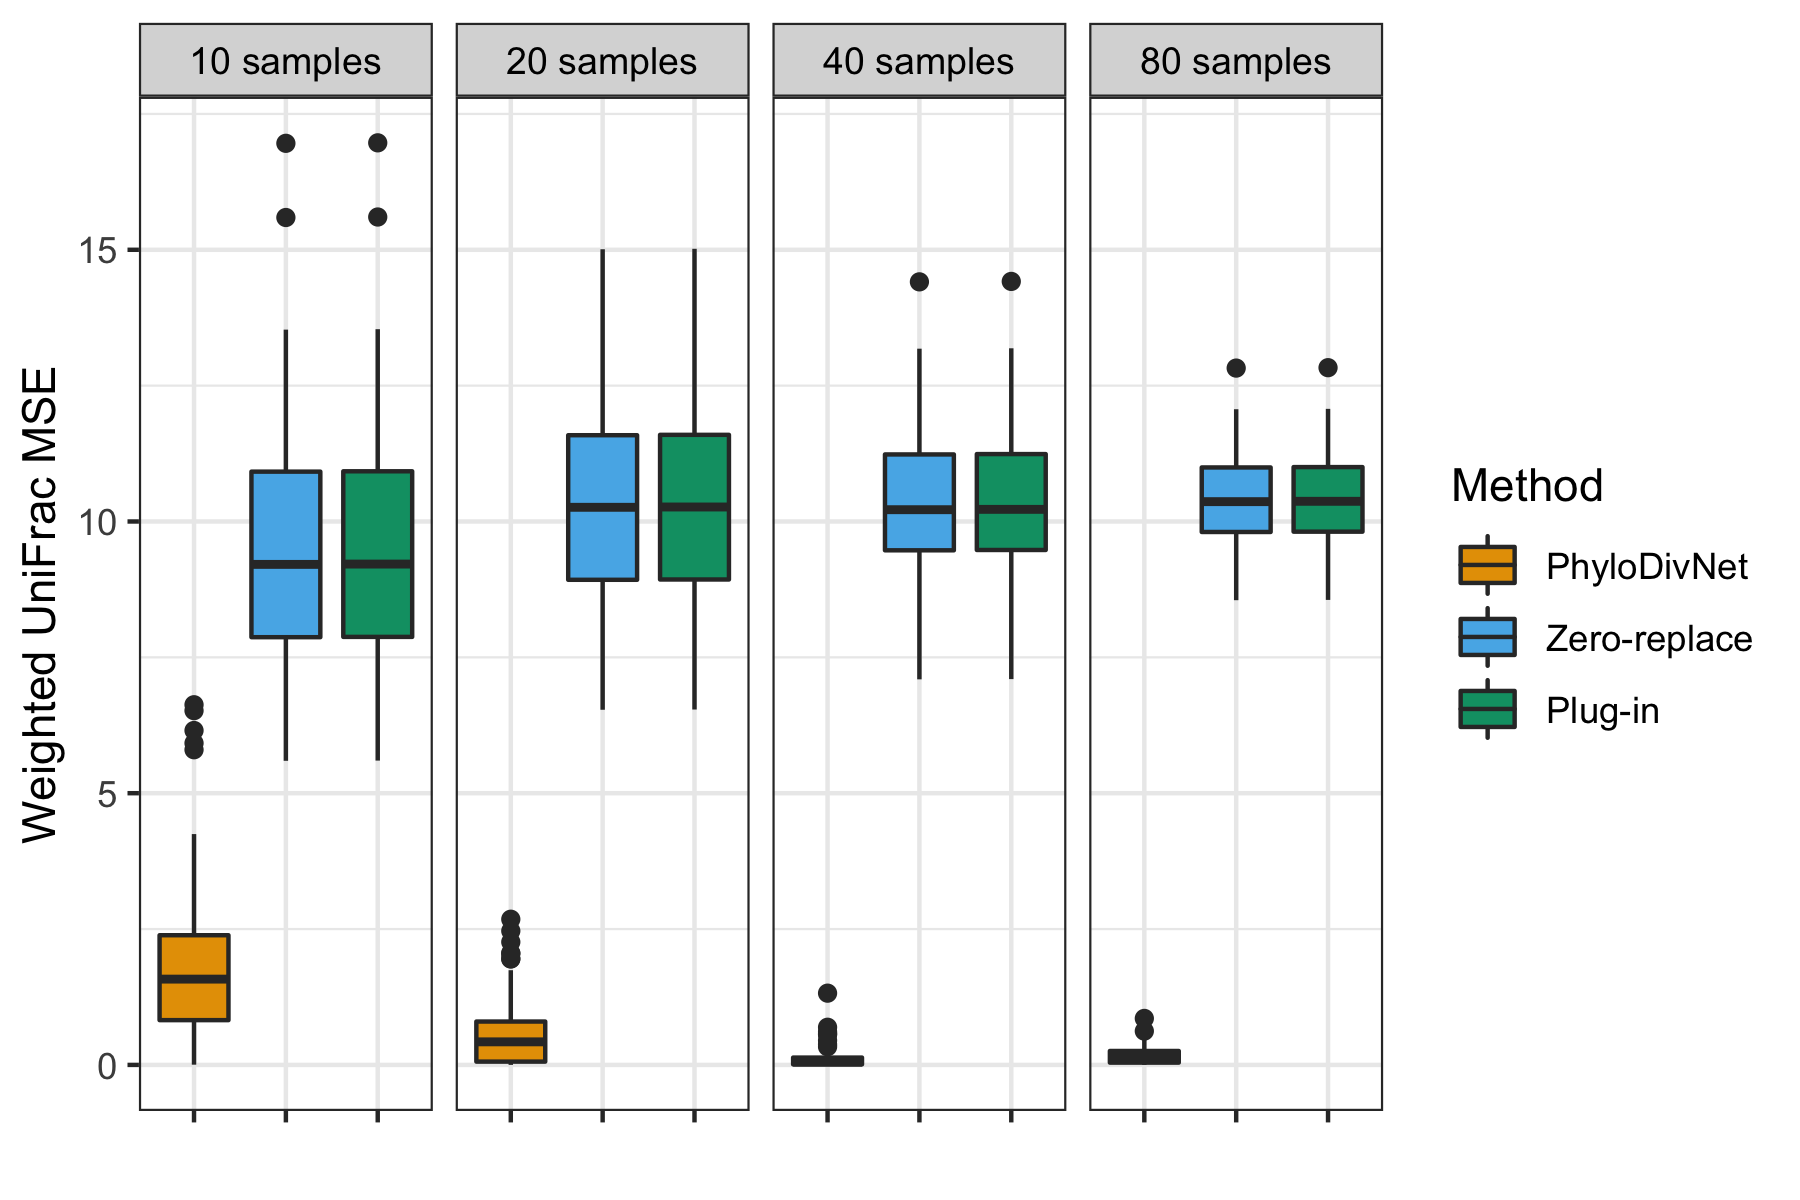
\includegraphics[width=\textwidth]{n_vary.png}
\end{figure}

Figure 1 illustrates the performance of {\myfont PhyloDivNet} against the \textit{zero-replace} and \textit{plug-in} estimators using the MSE. Increasing sample size results in lower estimation error when using {\myfont PhyloDivNet}, but the same pattern does not hold for the \textit{zero-replace} and \textit{plug-in} estimators. This is expected as these estimators do not utilize information from the covariate matrix in their estimation approaches and thereby do not benefit from the increased information afforded with larger sample sizes. Additionally, for all values of $n$ we see that the estimation error of {\myfont PhyloDivNet} is uniformly lower than the estimation error of the \textit{zero-replace} and \textit{plug-in} estimators.  These results are consistent with {\myfont DivNet}'s estimation of non-phylogenetic $\alpha$ and $\beta$ diversity metrics (Willis and Martin [Under Review]).

\subsection{Estimation Error is Small and Stable With Increasing Number of Taxa}
We next investigate the performance of {\myfont PhyloDivNet} against the \textit{zero-replace} and \textit{plug-in} estimators with varying number of taxa. For these simulations we set $n = 30$, $\sigma_{min} = 0.01$, $\sigma_{max} = 5$, $M_{i} = 10^5$ for all $i$, $K$ = 50 simulations, and evaluate four different community sizes $Q = 20, 50, 150, 300$. An input phylogenetic tree for each simulated set of $Q$ was constructed using the {\myfont rtree} function from {\myfont ape} (Paradis 2004) where $Q$ taxa are specified and the edges of the tree are randomly split until $Q$ tips have been reached. The branch lengths of the tree are drawn from a Uniform(0,1).

\begin{figure}[!htb]
 \captionsetup{singlelinecheck = false, format= hang, justification = raggedright, font = sf, labelsep = space}
  \caption{Normalized Weighted UniFrac: Q-vary}
  \centering
  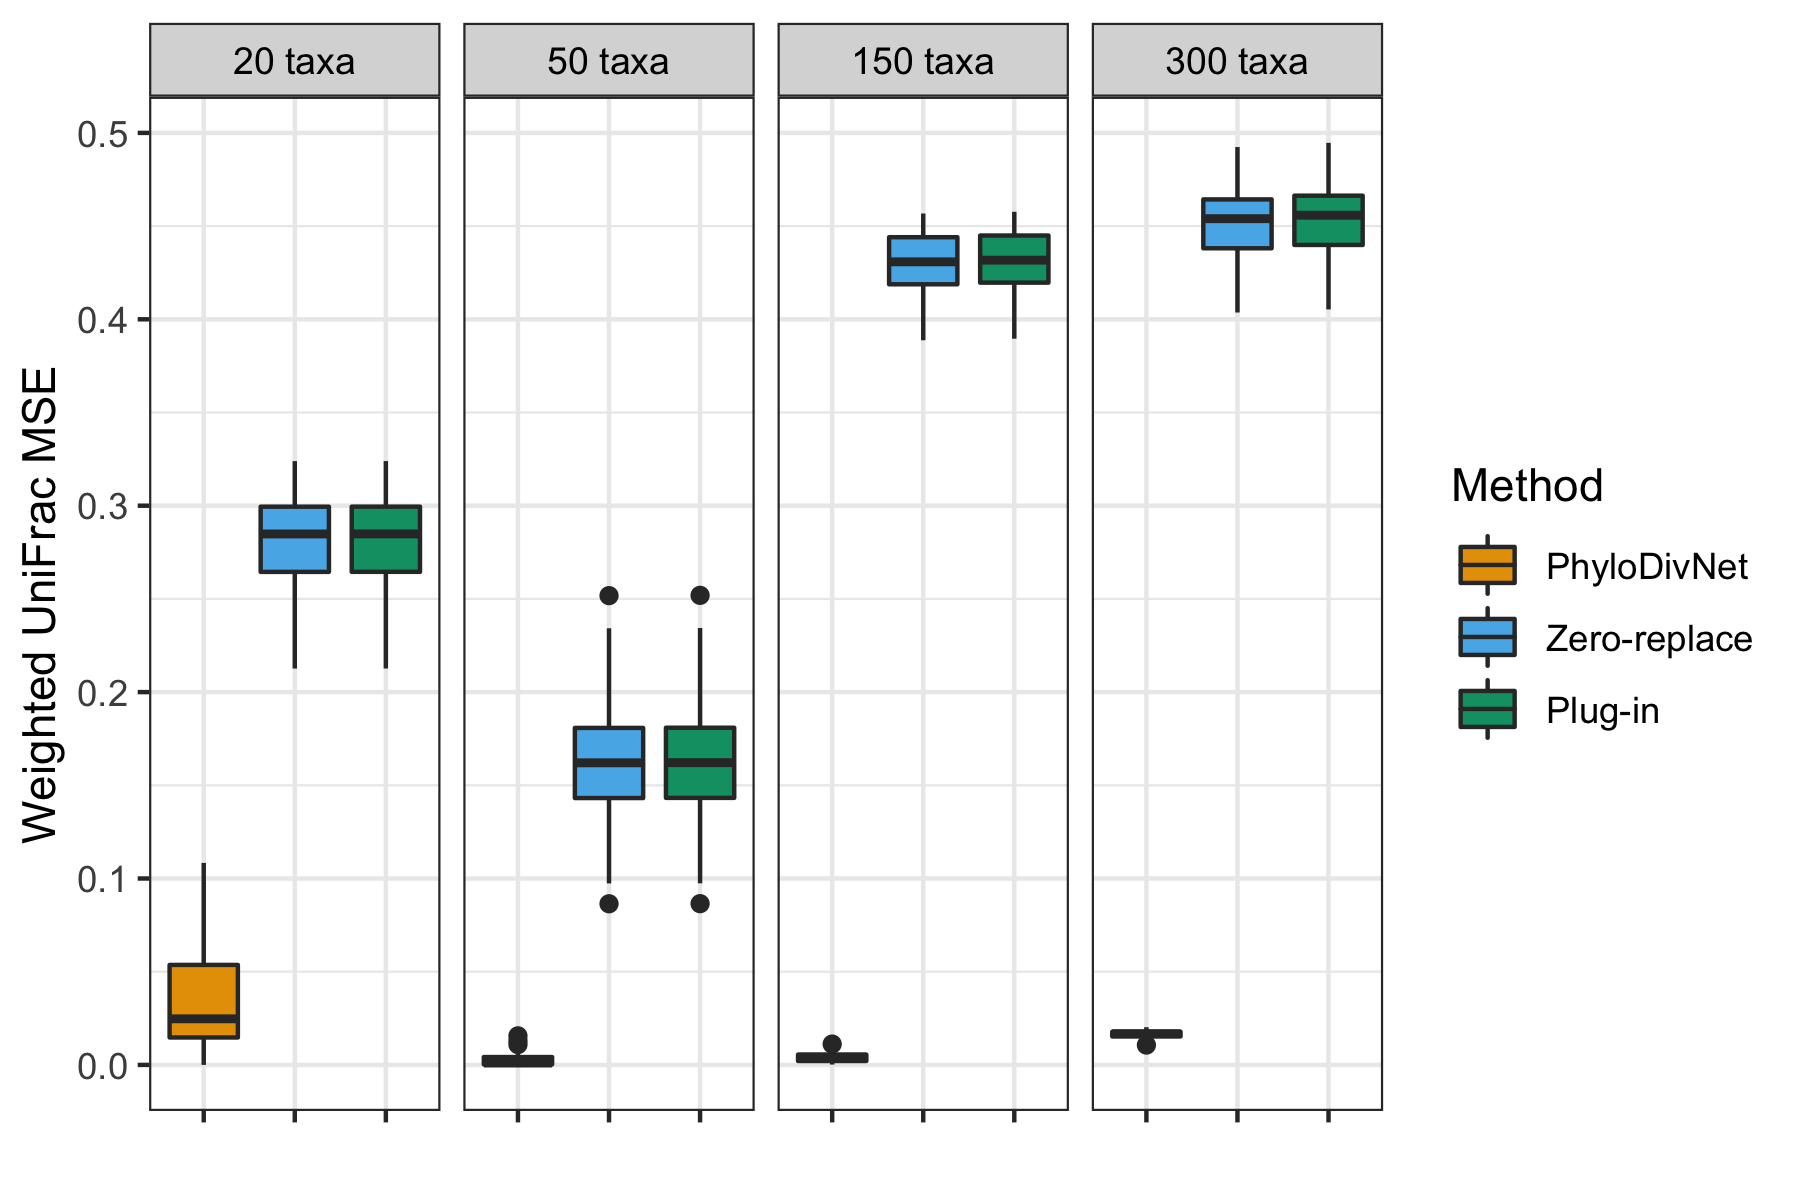
\includegraphics[width=\textwidth]{q_vary.png}
\end{figure}

Figure 2 shows the simulation results. We see that with increasing number of taxa {\myfont PhyloDivNet} maintains smaller estimation error than both the \textit{plug-in} and \textit{zero-replace} estimators. In fact, in all community sizes the 75th quantiles of ${MSE(\widehat{UniFrac}^{(k)})}_{k}$ for {\myfont PhyloDivNet} are uniformly lower than the \textit{zero-replace} and \textit{plug-in} methods. It common in microbiome studies for $q >> n$ and we see that estimation error is typically larger with larger numbers of taxa for the \textit{plug-in} and \textit{zero-replace} methods. Here we demonstrate that {\myfont PhyloDivNet} outperforms the \textit{zero-replace} and \textit{plug-in} methods in estimating the weighted UniFrac in terms of the MSE even in communities with large numbers of taxa.

\subsection{Estimation Error is Small and Stable Across Increasing Strengths of Co-occurrences}
We know that bacteria live in networked communities and that co-occurrence patterns exist between microorganisms that may be due to factors such as shared physiologies, habitat affinities, or functional ecological roles (Barber\'an et al. 2012). As such, a method for estimating diversity that can take into consideration co-occurrences would be appropriate for microbial community analysis. We investigate the estimation performance of {\myfont PhyloDivNet} with differing networks of microbial co-occurrences by examining different $\sigma_{max}$. $\sigma_{max}$ refers to the maximum eigenvalue of a $\Sigma$ matrix where larger eigenvalues correspond to stronger co-occurrences. For our simulations we set $Q = 50$, $n = 30$, $\sigma_{min} = 0.01$, $M_{i} = 10^5$ for all $i$, $K$ = 100 simulations, and evaluate four strengths of co-occurrences $\sigma_{max}$ = 0.1, 5, 10, 15. An input phylogenetic tree is constructed for each simulated set of $\sigma_{max}$ was constructed using the {\myfont rtree} function from {\myfont ape} (Paradis 2004) where $Q$ taxa are specified and the edges of the tree are randomly split until $Q$ tips have been reached. The branch lengths of the tree are drawn from a Uniform(0,1). Figure 3 displays the results of our simulation.
\begin{figure}[!htb]
 \captionsetup{singlelinecheck = false, format= hang, justification = raggedright, font = sf, labelsep = space}
  \caption{Normalized Weighted UniFrac: Sigma-vary}
  \centering
  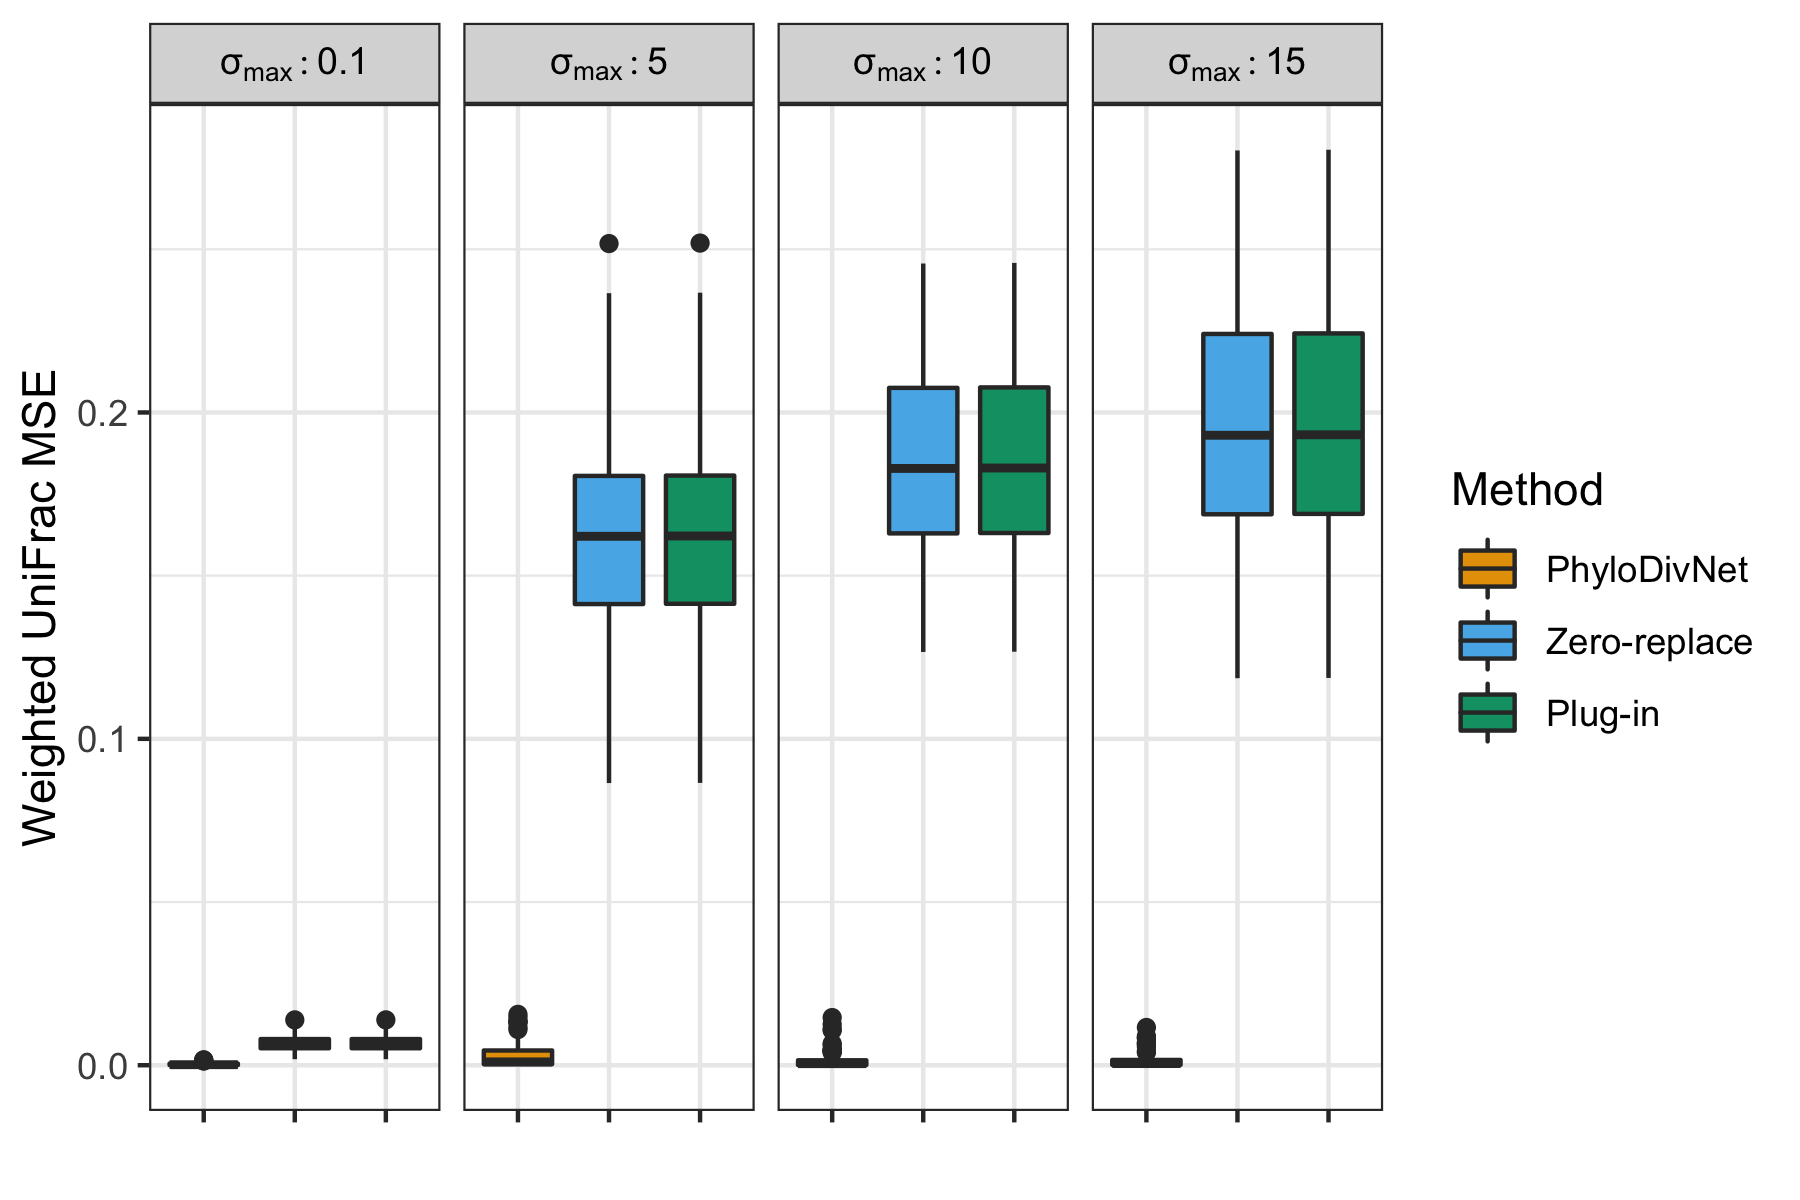
\includegraphics[width=\textwidth]{s_vary.png}
\end{figure}

We observe that with stronger co-occurrences the estimation error increases for the \textit{zero-replace} and \textit{plug-in} estimators whereas {\myfont PhyloDivNet}'s estimation error remains consistently smaller. We thus conclude that {\myfont PhyloDivNet} is well suited for estimating weighted UniFrac in the presence of strong and weak microbial co-occurrence networks.

\subsection{Estimation Error is Small and Stable for Balanced and Unbalanced Trees}
Weighted UniFrac is a phylogenetic quantitative $\beta$-diversity measure that uses relative abundance information to weight the branch lengths of the tree in its calculation of distances between ecosystem $i$ and $j$. There are two distinct features of rooted phylogenetic trees. First the topology of the tree and secondly the branch lengths which correspond to periods of time separating evolutionary events. The shape of a tree carries useful information about diversification rates among species. One of the most widely used indices to measure tree balance is Colless' index which looks at each internal node indexed by $j = 1,...,n-1$ for a phylogenetic tree with $n$ tips and partitions the leaves that descend from each $j$ node into $L_j$ and $R_j$ sized groups. The absolute difference between $L_j$ and $R_j$ is calculated at each node and summed across all nodes to compute the Colless metric.

\begin{equation}
  I_c = \sum_{j=1}^{n-1}|L_j-R_j|
\end{equation}

A standardization of the Colless metric under the Yule model allows for comparison across different tree sizes. Under the Yule model the standardized Colless index is
\begin{equation}
  I_{yule} = \frac{I_c - n * log(n) - n(\gamma - 1 - log(2))}{n}
\end{equation}
where $\gamma$ is the Euler constant. A value of $I_c$ equal to 0 represents a balanced tree and as follows the larger the positive value the greater the imbalance. Therefore more negative values of $I_{yule}$ represent more balanced trees and more positive values reflect more imbalanced trees. To investigate the performance of {\myfont PhyloDivNet} on balanced versus balanced phylogenetic trees we simulate a set of 10,000 Yule trees using {\myfont phytools} (CITE) fixing $q = 60$ tips. Because the Yule process assumes that every lineage is equally likely to speciate at any given time with no extinction and only birth until $q$ tips are reached, the phylogenetic trees generated are ultrametric.

To evaluate our method on balanced and unbalanced tree topologies we calculated the Yule standardized Colless metric for all 10,000 trees and defined balanced trees as $I_c < -1$ and unbalanced trees as $I_c > 1$. This yielded 1000 trees of our 10,000 simulated trees that were considered unbalanced and 1000 trees that were considered balanced. We designated the tree with the lowest Colless statistic as the true balanced tree and similarly the tree with the highest Colless statistic as the true unbalanced tree. Of the remaining trees we randomly drew without replacement from our pool of unbalanced and balanced trees for use in our simulations. We set $n = 40$, $ p = 3$, $\sigma_{max} = 5$, $\sigma_{min} = 0.01$, $M_{i} = 10^5$ for all $i$, K = 50 simulations. Figure 5 shows the simulation results.

\begin{figure}[!htb]
    \centering
    \captionsetup{singlelinecheck = false, format= hang, justification = raggedright, font = sf, labelsep = space}
    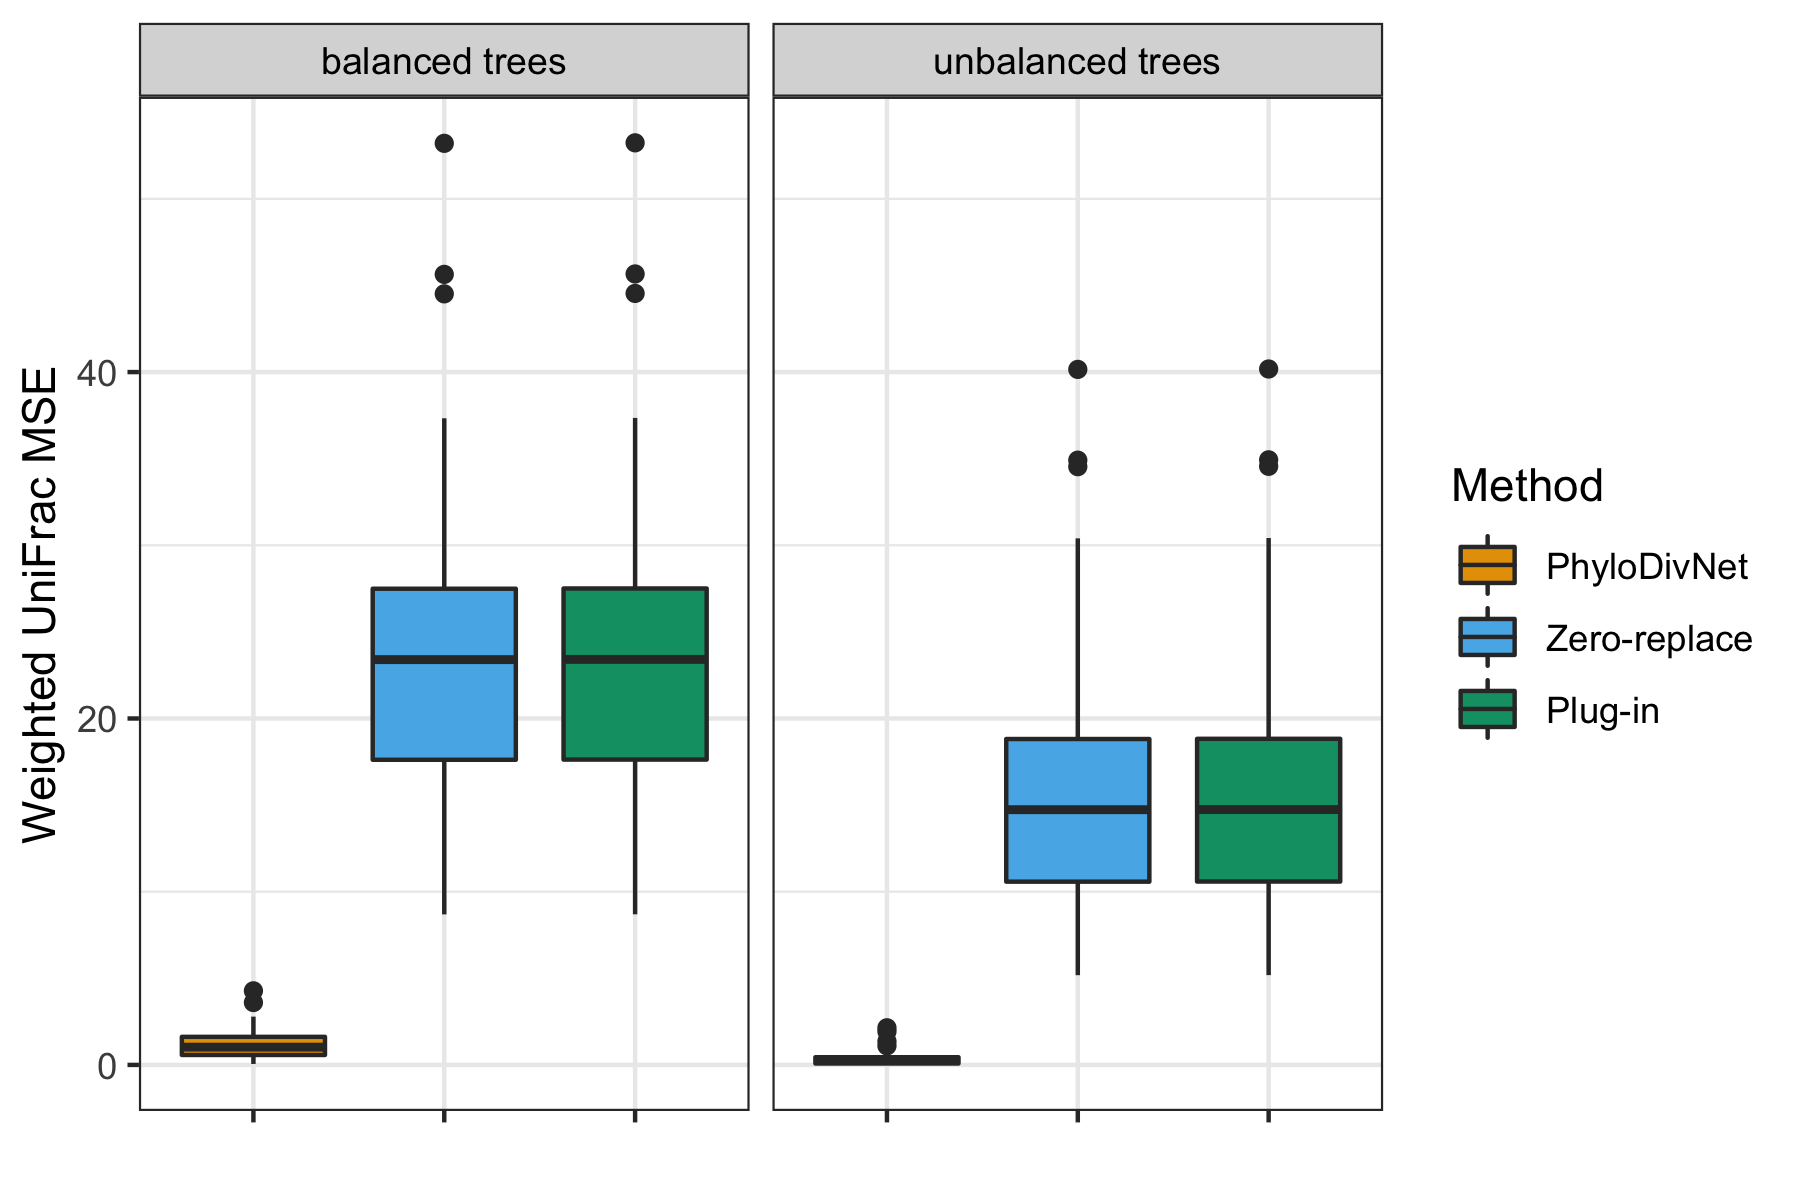
\includegraphics[width=\textwidth]{tree_vary.png}
    \caption{Weighted UniFrac: Unbalanced vs. Balanced Trees}
    \label{fig:my_label}
\end{figure}

In Figure 5 we see that estimation error is small and stable for our proposed method compared to the \textit{plug-in} and \textit{zero-replace} methods for both balanced and unbalanced tree shapes.

\textbf{Note: Amy, as I as going through this section I am dissatisfied with how I did these phylogenetic tree simulations and I believe I can do better. I had several thoughts (1) You had suggested that I bin the Colless metric so that I didn't choose an arbitrary cut-off point for balanced/unbalanced trees but I wasn't actually sure what would be considered the ``true tree'' for each Colless interval so I left it the way it is currently until I talked about it with you a bit more in April. (2) building on that, I was delving into the phylogenetic tree simulation package TreeSim and thinking about how phylogenetic trees are constructed and how that might affect weighted UniFrac, I think I could do a better job with testing different phylogenetic trees not based on the balanced vs unbalanced design but maybe based on evolutionary rate and extinction rate. I'd like to think about simulating a birth-death tree (which will get me non ultrametric trees) so I wanted to make this my first task coming back that first week to improve on this section.}

\section{Data Analysis: Healthy Dairy Worker Study}
The Healthy Dairy Worker (HDW) study is a on-going cohort study that explores the health effects of microbial exposures from a dairy farm on dairy workers in the Pacific Northwest. One of the primary aims of the study is to understand the microbial sharing that occurs between dairy workers, dairy cows, and the dairy farm environment. The study thus provides an especially relevant setting to understand differences in community composition between cows, workers, and the environment through the use of weighted UniFrac. By January 2019, fecal samples for 38 dairy workers and 14 dairy cows as well as 22 environmental swabs were collected at baseline. DNA was extracted using MoBio DNeasy PowerLyzer PowerSoil Kits. Library prep was performed according to the Earth Microbiome Project (EMP) protocol (CITE EMP) and samples were sequenced using an Illumina MiSeq targeting the V4 region of the 16s rRNA subunit.

Paired end sequences were processed using DADA2 (Callahan et al. 2015). First, primer sequences were filtered and trimmed from forward and reverse reads. Based on quality scores of 20 or greater, forward sequences were trimmed left at nucleotide position 20 and truncated right at position 200. Reverse reads were trimmed left at position 50 and truncated right at position 200. Paired end sequences were then merged and chimeras removed to create a table of amplicon sequence variants (ASVs) and their counts. A phylogenetic tree was then constructed using SAT\'{e}-enabled phylogenetic placement (SEPP) (Mirarab et al. 2012). SEPP allows for phylogenetic tree construction by inserting sequences into a reference phylogeny and thereby creating trees with more accurate branch lengths than those generated using de novo phylogeny reconstruction (Janssen et al. 2018). The reference phylogeny and matching alignment used in this analysis was Greengenes $13\_8$ at $99\%$ (CITE). The ASV table was then filtered to include only the fragments that were present in the insertion tree. A final filtering of the data was done using a minimum ASV abundance cutoff of 0.005\% of total reads as is recommended when a mock community is not incorporated in sequencing to minimize the generation of spurious ASVs (Bokulich et al. 2013). A total of 3,441 amplicon sequence variants (ASV) remained after quality filtering and processing for analysis. Data processing was done using R 3.5.0 and q2-fragment-insertion (Janssen et al. 2018).

\textbf{[INSERT HERE: Investigating the different choices of D (reference taxon) and Amy's plot idea of the continuous UniFracs along a phylogenetic tree for each taxon selected as the reference]}

We compare our proposed method {\myfont PhyloDivNet} with the \textit{zero-replace} and \textit{plug-in} methods for estimating weighted normalized UniFrac. We use the most abundant taxon as the reference taxon $D$ (Eq.6). A parametric bootstrap approach as described in Section 2.3 is used to estimate the variance with $B$ = 100. The results are displayed in Figure 6 with the 25\% and 75\% quantiles shown.

\begin{figure}[!htb]
 \captionsetup{singlelinecheck = false, format= hang, justification = raggedright, font = sf, labelsep = space}
  \caption{Data Analysis Results}
  \centering
  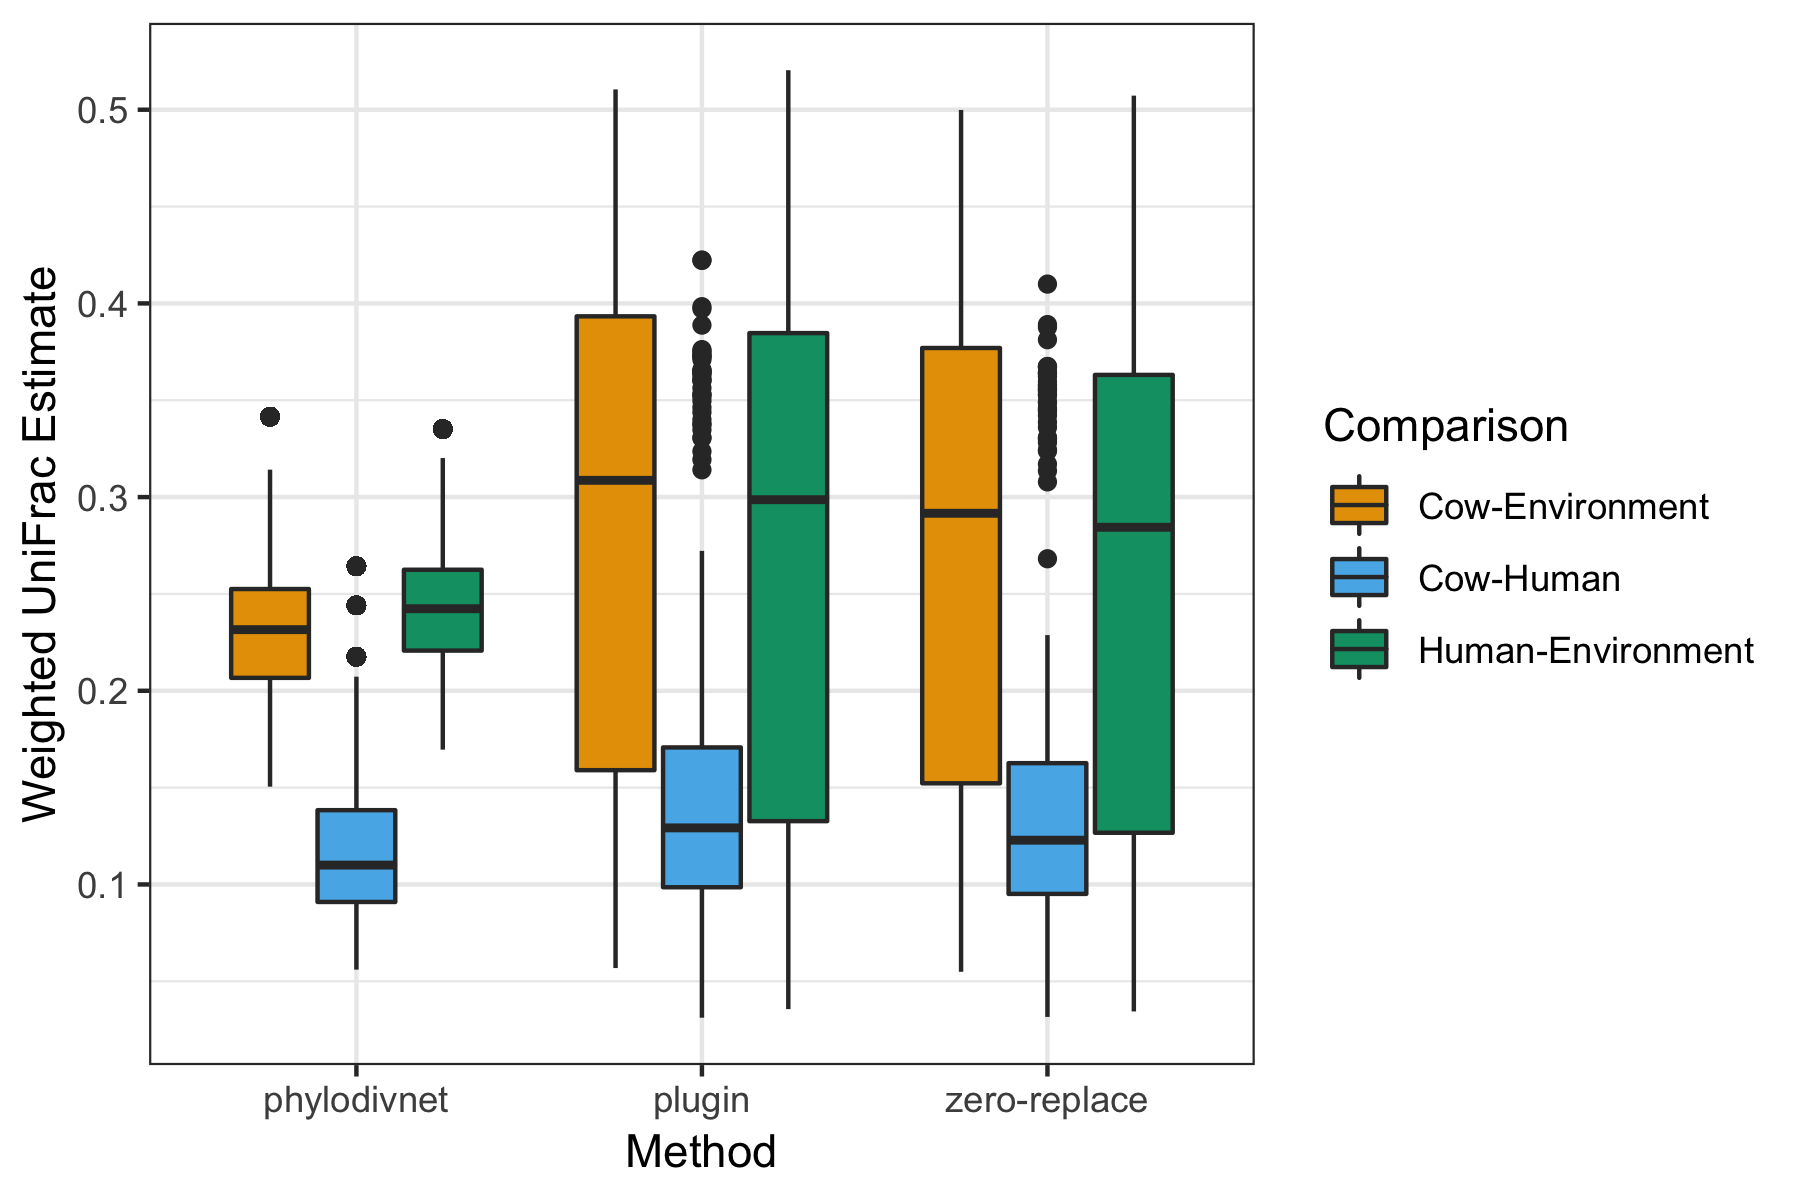
\includegraphics[width=\textwidth]{HDWanalysis_plots_B100_3methods.png}
\end{figure}

Comparing the weighted UniFrac estimates in Figure 6 generated by each method, we see that the intervals for {\myfont PhyloDivNet} are smaller than the intervals for the \textit{plug-in} and \textit{zero-replace} methods. Additionally our method produces interval estimates that are more symmetric around the median than the comparison methods. Another noted advantage of our method compared to the \textit{plug-in} and \textit{zero-replace} methods is the use of multiple covariates in estimating the weighted UniFrac.

\section{Hypothesis Testing}
- hypothesis testing evaluation section here


\section{Discussion}
\begin{itemize}
  \item  Discuss the idea that groups of people based on some design matrix/covariates can be considered replicates in the same way that we do with other regression methods when testing for differences between groups
  \item Why we didn't estimate unweighted UniFrac
  \item  Emphasize the importance of type 1 error control and hypothesis testing
\end{itemize}

\section{Conclusion}
\begin(itemize)
  \item
\end{itemize}


{\myfont github.com/statdivlab/PhyloDivNet}


\bibliographystyle{plain}
\bibliography{references}
Mart\'in-Fern\'andez 2003 https://link.springer.com/content/pdf/10.1023%2FA%3A1023866030544.pdf

Vu 2007
https://statistics.berkeley.edu/sites/default/files/tech-reports/727.pdf

Paradis 2004
https://cran.r-project.org/web/packages/ape/index.html

Barber\'an https://www.ncbi.nlm.nih.gov/pmc/articles/PMC2728295/

\end{document}
